\documentclass[10pt,a4paper, twocolumn]{article}
\usepackage[utf8]{inputenc}
\usepackage[english]{babel}
\usepackage{amsmath}
\usepackage{amsfonts}
\usepackage{amssymb}
\usepackage{graphicx}
\usepackage{mathtools, cuted}
\usepackage{widetext}

\begin{document}


\title{Beyond Boost-invariant Initial Condition for Relativistic Heavy Ion Collision simulation}
\author{Weiyao Ke}
\maketitle


\abstractname{:}

\section{Introduction}
	\subsection{Relativistic Heavy Ion Collision}
	Ultra-relativistic heavy ion collision produces the hottest medium in the lab since the first operation of RHIC at Brookhaven National Lab. 
	The transient hot and dense state of matter with a life time of femtoseconds is known as quark-gluon plasma (QGP). 
	Viscous hydrodynamics modelling with thermalization at early stages very well describes the experimental data. 
	An unexpectedly low shear viscosity to entropy ratio $\eta/s$, close to the quantum lower bound from AdS/CFT correspondence, is needed to explain the observed momentum anisotropy.
	The system therefore behaves like an almost perfect liquid, revealing the strongly coupled nature of the problem.
	This motivates large effort to quantify the transport properties of this new state of matter.
	
	Modelling is essential to the problem. 
	Since quarks and gluons always hadronize and what can be detected directly are hadrons and decay products, it requires modelling time evolution of both QGP and hadron final states in order to compare with experimental data. 
	Also, due to the lack of knowledge of initial stages of the collision such as nuclear wave function and how the system undergoes fast thermalization and isotropization, models of initial condition are indispensable.
	
	\subsection{Soft and Hard Observables}
		
	
	\subsection{``Standard Model" of Soft Physics}
	The present "Standard Model" of soft sector in relativistic heavy ion collision consists of four stages.
	\begin{itemize}
		\item Fast thermalization. 
		Immediately after the collding of two nuclei, the fireball is far from thermal equilibrium. However, in less than $1 \textrm{ fm/c}$, the system is already close to local thermal equilibrium. 
		The reason of this fast thermalization is still not clear.
		\item Hydrodynamical expansion of QGP. 
		Relativistic viscous hydrodynamics describes the expansion of QGP by solving energy-momentum and charge conservation,
		\begin{eqnarray}
			\partial_\nu T^{\mu\nu} &=& 0, \\
			\partial_\nu N^{\nu} &=& 0. 
		\end{eqnarray}
		Hydrodynamics translates initial spatial anisotropy into momentum space anisotropy reproducing the famous harmonic flows. 
		Equation of state of hot QCD matter is an input as calculated from Lattice QCD.

		\item Statistical hadronization, freezeout. 
		As temperature drops and hydrodynamics does not apply, the system is particularized by statistical sampling hadrons from particle distribution function, the Cooper-Frye formula,
		\begin{eqnarray}
			E\frac{\mathrm{d}N_i}{\mathrm{d}^3p} = \int_\Sigma f_i(x, p)p^\mu,\mathrm{d}^3\sigma_\mu.
		\end{eqnarray}
		\item Final state scattering. 
		The system after freezeout is still dense enough to allow hadronic scattering. 
		Transport model such as UrQMD is utilized to solve the Boltzmann equation,
		\begin{eqnarray}
			\frac{\mathrm{d}f_i(x, p)}{\mathrm{d}t} = C_i(x, p).
		\end{eqnarray}
	\end{itemize}

\section{Boost-invariant Approximation and TRENTo IC}
	The matter produced in heavy ion collision expand rapidity in the beam direction. So it is convenient to express the system in terms of curvilinear coordinates $(\tau, x, y, \eta_s)$. 
	With $x, y$ remains the same as Cartesian coordinates transverse to beam direction, $\tau$ and $\eta_s$ are known as local time and space-time rapidity of the system,
	\begin{eqnarray}
		\tau = \sqrt{t^2 - z^2} &,& \eta_s = \frac{1}{2}\ln\left(\frac{t+z}{t-z}\right) \\
		t = \tau \cosh \eta_s &,& z = \tau \sinh \eta_s.
	\end{eqnarray}
	These coordinates transforms under lorentz boost along $z$ direction as,
	\begin{eqnarray}
		(\tau, {\bf x_{\perp}}, \eta_s) \xrightarrow{L} (\tau, {\bf x_{\perp}}, \eta_s + \Delta)
	\end{eqnarray}
	
	A boost invariant solution of hydrodynamics is a solution without $eta_s$ dependence, therefore the solution looks the same in every frame related by a boost along beam axis. 
	For example, when nuclei are modelled by infinitely large uniform slab in transverse direction, the boost invariant solution in curvilinear frame $\tau s = const.$ recast into Cartesian coordinates,
	\begin{eqnarray}
		s = \frac{const.}{\sqrt{t^2 - z^2}}.
	\end{eqnarray}
	Under the boost-invariant approximation, it is sufficient to specify the initial condition at mid-rapidity ($\eta_s = 0$). Various models were proposed to describe the entropy/energy deposition at mid-rapidity. 
	However, these models can be phenomenologically described with an effective model TRENTo.
		
	TRENTo IC consist of three levels of parametrization,
	\begin{itemize}
		\item Binary nucleon-nucleon collision.
		\item Nuclear-nuclear collision.
		\item Mid-rapidity entropy deposition ansatz.
	\end{itemize}
	The first two steps are similar to the procedures of Monte-Carlo Glauber Model; however, TRENTo employs a much generalized entropy deposition formula.
	\subsection{Parametrization of Binarg Nucleon-nucleon collision}
	Impact parameter differential inelastic cross-section is parametrized in the eikonal limit,
	\begin{eqnarray}\label{dsigma_db}
		\frac{\mathrm{d}\sigma_{nn}}{2\pi b \mathrm{db}} = 1 - \exp\left(-\alpha T_{pp} (b)\right).
	\end{eqnarray}
	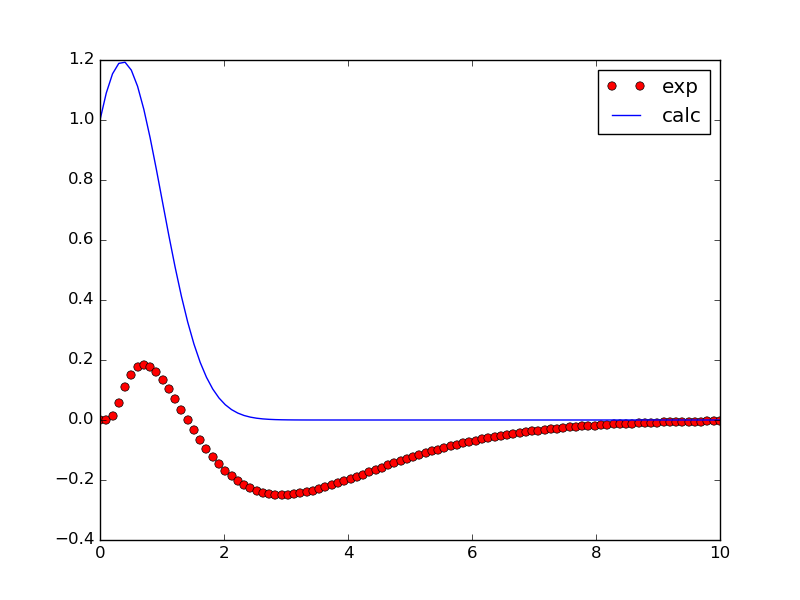
\includegraphics[width=\columnwidth]{pics/place_holder.png}
	$T_{pp}$ is the overlapping of nucleons' transverse density function $\rho(x_\perp)$, which is generally assumed to be normalized Gaussian,
	\begin{eqnarray}
		\rho(x_\perp) &=& \frac{1}{\sqrt{2\pi w^2}}\exp\left(-\frac{{x_\perp}^2}{2w^2}\right), \\
		T_{pp}(b) &=& \int \mathrm{d}{x}^2 \rho(x+\frac{b}{2})\rho(x-\frac{b}{2})
	\end{eqnarray}
	All the information of subnucleonic degrees of freedom is encoded in the coefficient $\alpha$, which is tuned to reproduce the inelastic proton-proton inelastic cross-section at a given energy,
	\begin{eqnarray}
		\int \mathrm{d}\sigma_{nn}(\alpha) = \sigma_{pp, inel}(\sqrt{s}).
	\end{eqnarray}
	Eq. (\ref{dsigma_db}) is then interpreted as the probability for two nucleon to collide with separation of $b$ and is realized via a Monte Carlo approach.
	\subsection{Parametrization of Nuclear-nuclear Collision}
	The penetrating of nuclei of ultra-relativistic collision takes much shorter time than the time scale of nucleon motion inside a nuclei; therefore, nucleon position fluctuation need to be taken into account. 
	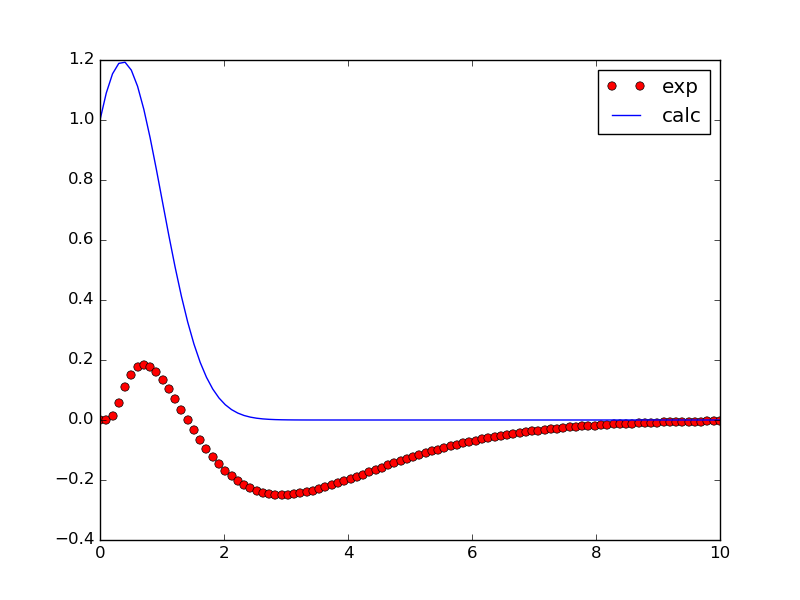
\includegraphics[width=\columnwidth]{pics/place_holder.png}
	In TRENTo, nucleons are sampled from a (deformed) Woods-Saxon density distribution and then projected onto the transverse plain. 
	Each pair of nucleons with one from projectile and the other from target nuclei is examined with the binary collision criterion. 
	Nucleons subject to at least one collision are called participants, and the rest, spectators.
	The contribution of participants from nuclei $\{A,B\}$ defines the nuclear thickness function:
	\begin{eqnarray}
		T_{A,B}(x_\perp) &=& \sum_{i \in Part A,B} \gamma_i. \rho(x_\perp- x_i), \\
		\gamma_i &\sim& \Gamma(k, k).
	\end{eqnarray}
	Note that the contribution from each participant nucleon is multiplied by a random variable $\gamma_i$ subject to $\Gamma$ distribution with unity mean and variance $1/k$. 
	This additional source of fluctuation is added to reproduce the negative binomial distribution of number of charged particle in minimum biased $pp$ collisions.
	\subsection{Entropy Deposition Ansatz}
	TRENTo assumes in the eikonal limit, immediately after the penetrating of the nuclei, entropy deposition are local function of nuclear thickness functions $T_{A,B}$. 
	Generalized mean ansatz provide a flexible way to parametrize this mapping,
	\begin{eqnarray}
	\left.\frac{\mathrm{d^3}s}{\mathrm{d}\eta_s \mathrm{d}x_\perp^2}\right\vert_{\eta_s = 0} &=& 	T_R\left(T_A, T_B; p\right),	\\
	T_R(x, y; p) &=& \left(\frac{x^p+y^p}{2}\right)^{\frac{1}{p}}.
	\end{eqnarray}
	With parameter $p$ various, this ansatz mimic a variety of initial condition models.
	\begin{center}
	\begin{tabular}{c|c|c|c}
	\hline
	$p$	&	$-0.5$	 	&	$0.0$ 		& 	$1.0$		\\
	\hline	
	$\sim$ &		KLN		& 	EKRT		& 		Wounded Nucleon \\
	\hline
	\end{tabular}
	\end{center}
	The ``$\sim$" sign in the table reminds that $T_R$ resembles the entropy deposition of different models for reasonable value of thickness function. 
	This parametrization allows interpolation between different initial condition models and is suitable for a model selection procedure to learn what is the most probable initial condition to explain the observed experimental data at mid-rapidity.
	A model to data comparison by Bayesian analysis has very well constrained $p$ to be close to zero.
\section{Rapidity Dependent Extension of TRENTo}
	Instead of getting lost with arbitrary functions $f(\eta)$ to implement rapidly dependent hydrodynamic initial condition and at the same time systematically controls key behaviours of the parameterization, we reconstruct the entropy rapidity distribution locally from its cumulants generating function. 
	The mean $\mu$, the standard deviation $\sigma$ and the skewness $\gamma\sigma^3$ constitute the three most involved set of cumulants. 
	We utilise what is found in section 3 and assume that at each transverse point with nuclear thickness function $T_A(x{\perp})$ and $T_B(x{\perp})$,
	\begin{eqnarray}
		\mu(x_\perp) &=& \frac{1}{2}\ln(\frac{T_A(x_\perp)}{T_B(x_\perp)}), \\
		\sigma(x_\perp) &=& 2.5 \sim 3.0, \\
		\gamma(x_\perp) &=& \gamma_0 (T_A(x_\perp) - T_B(x_\perp)) \mathrm{fm}^2. \\
	\end{eqnarray}
	In this way, the rapidity distribution at each $x_\perp$ is a distribution centering at the centre of mass rapidity $\eta_{cm} =  \frac{1}{2}\ln(\frac{T_A(x_\perp)}{T_B(x_\perp)})$, with a fixed standard deviation $\sigma$ and a skewness promotional to the difference in the nuclear thickness function (in units of fm${}^2$).
	It is also required the mid-rapidity entropy production is normalised to the generalised mean ansatz so that the mid-rapidity prediction of the model is intacted,
	A model to data comparison at mid-rapidity, LHC energies suggests that $p \sim 0$, which reduces the generalised mean to $T_R (p \rightarrow 0) = \sqrt{ T_A(x_\perp) T_B(x_\perp) }$.
	
	With these information, the pseudorapidity distribution can be reconstructed by inverse Fourier transform of cumulant generating function:
	\begin{eqnarray}
		\frac{\mathrm{d}S}{\mathrm{d}x_{\perp}^2 \mathrm{d}\eta}  &\propto& T_R(x_\perp) \frac{F(x_\perp,y)}{F(x_\perp,y = 0)}\frac{\mathrm{d}y}{\mathrm{d}\eta}, \\
	 	F(x_\perp,y) &=& \mathcal{F}^{-1}\{\tilde{F}(k)\} \\
	 	\ln \tilde{F} &=&  i \mu k - \frac{1}{2}\sigma^2 k^2 + i 	\gamma k^3  - \kappa k^4
	\end{eqnarray}
	with the relation between rapidity and pseudorapidity,
	\begin{eqnarray}
		\eta &=& \sinh^{-1}(\sqrt{K}\sinh(y)),\\ 
		K &=& \left< 1+ \frac{{p_T}^2}{{m_T}^2} \right>
	\end{eqnarray}
	
	Different models can be mapped to different parametrization of cumulants,
	
	\begin{strip}
	\begin{center}
	\begin{tabular}{c|c|c|c|c}
	\hline
	--	&	$\mu(x_\perp)$ & $\gamma(x_\perp)$ & $\sigma(x_\perp)$ & $\kappa(x_\perp)$	\\
	\hline
	shifted & $\frac{1}{2}\log\left(\frac{T_A}{T_B}\right)$ & $0$	& const. & const.\\
	tilted & $0$ & $T_A - T_B, \frac{T_A-T_B}{T_A+T_B}, etc$	& const.& const.\\
	general & $\frac{a}{2}\log\left(\frac{T_A}{T_B}\right)$  & $b(T_A - T_B)$ & const.& const. \\
	\hline
	\end{tabular}
	\end{center}
	\end{strip}
	However, it turns out, for the range of $\gamma$ encountered in p + Pb collisions ($\gamma \sim 0-2$, to be shown later), the inverse transform function is not well-behaved for relatively large $\gamma$. 
	As can be seen from Fig. \ref{regularization}, left panel, the function constructed with the first three cumulant. 
	The truncated generating function yield a distribution that begins to lose control and goes negative at large $|\eta|$ with increasing $\gamma$. 
	This shows the importance of including higher order cumulants to regularize the behaviour of the generating function. 
	The constrains on functions which yields positive definite real Fourier transform are quite involved, but we find in the present case, the following replacement works, even not perfect,
	\begin{eqnarray}
		\{\gamma, \kappa\} \rightarrow \{\gamma, \kappa\} \exp\left(-\frac{1}{2}\sigma^2k^2\right) 
	\end{eqnarray}
	Compared to its predecessor, terms systematically from higher order odd cumulants are included so that the contribution from the third term in the exponential is effectively suppressed for modulation faster than $1/\sigma$. 
	With these regularization procedure, skewness of the distribution remains unchanged; however the performance of its inverse Fourier transform is significantly improved as seen in Fig. \ref{regularization}, right panel. 
	The distribution reconstructed with regularization produce and is positive and well behaved over a wide range of rapidity and skewness.
	\begin{figure}[htbp]
		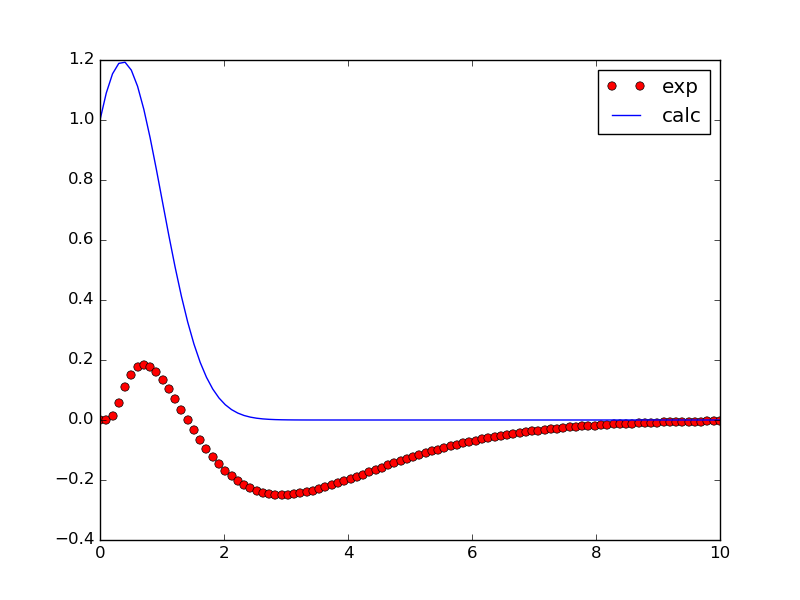
\includegraphics[width = \columnwidth]{./pics/place_holder.png}
	\caption{Effect of regularization.}
	\label{regularization}
	\end{figure}

\section{Model to Data Comparison}
	
\section{Results}
	\subsection{IC against Experiments}
	\subsection{Evolution Response and Observables}
\section{Outlook}

\section{Summary}

\end{document}